\documentclass[tikz,border=5pt]{standalone}
\usepackage[T1]{fontenc}
\usepackage[utf8]{inputenc}
\usepackage{lmodern}
\usepackage{amsmath,amssymb}
\usepackage{siunitx}
\usepackage{xcolor}
\usepackage{tikz}
\usetikzlibrary{
  arrows.meta,
  backgrounds,
  calc,
  decorations.pathreplacing,
  fit,
  matrix,
  positioning,
  shapes.geometric
}

\sisetup{
  detect-all = true,
  group-minimum-digits = 4,
}

\definecolor{TdcBlue}{HTML}{5B739F}
\definecolor{TdcRed}{HTML}{A35E66}
\definecolor{TdcLilac}{HTML}{8D83A7}
\definecolor{TdcCyan}{HTML}{82A9B8}
\definecolor{TdcGray}{HTML}{6D7175}
\definecolor{TdcBlack}{HTML}{202124}

\colorlet{TdcBlueFill}{TdcBlue!7}
\colorlet{TdcRedFill}{TdcRed!7}
\colorlet{TdcLilacFill}{TdcLilac!8}
\colorlet{TdcCyanFill}{TdcCyan!10}
\colorlet{TdcGrayFill}{black!3}
\colorlet{TdcGuide}{black!32}
\colorlet{TdcGuideLight}{black!18}

\tikzset{
  >=Latex,
  every picture/.style = {line join=round, line cap=round},
  every node/.style = {font=\small, text=TdcBlack},
  module/.style = {
    draw=black!72,
    fill=white,
    line width=0.50pt,
    rounded corners=0.8pt,
    minimum height=9mm,
    minimum width=22mm,
    align=center,
    inner sep=3pt
  },
  module gray/.style = {module, fill=TdcGrayFill},
  module slow/.style = {module, draw=TdcBlue, fill=TdcBlueFill},
  module fast/.style = {module, draw=TdcRed, fill=TdcRedFill},
  module ctrl/.style = {module, draw=TdcLilac, fill=TdcLilacFill},
  module io/.style = {module, draw=TdcCyan, fill=TdcCyanFill},
  domain box/.style = {
    draw=black!32,
    fill=black!1.5,
    line width=0.40pt,
    rounded corners=1.0pt,
    inner sep=4pt
  },
  domain label/.style = {
    font=\scriptsize\itshape,
    text=black!70
  },
  signal/.style = {-{Latex[length=2.2mm,width=1.5mm]}, draw=black!72, line width=0.60pt},
  signal slow/.style = {signal, draw=TdcBlue},
  signal fast/.style = {signal, draw=TdcRed},
  signal ctrl/.style = {signal, draw=TdcLilac},
  signal io/.style = {signal, draw=TdcCyan!80!black},
  signal dashed/.style = {signal, dashed},
  bidir/.style = {<->, draw=black!72, line width=0.55pt},
  guide/.style = {draw=TdcGuide, line width=0.35pt},
  guide dashed/.style = {guide, dashed},
  fine mark/.style = {draw=black!60, line width=0.40pt},
  brace note/.style = {
    decorate,
    decoration={brace, amplitude=3.0pt},
    draw=black!55,
    line width=0.40pt
  },
  note/.style = {
    font=\scriptsize,
    inner sep=1.5pt,
    fill=white,
    text=black!78
  },
  axis label/.style = {
    font=\scriptsize,
    text=black!72
  },
  lane label/.style = {
    font=\small,
    text=black!82
  },
  legend box/.style = {
    draw=black!60,
    line width=0.40pt,
    minimum width=4mm,
    minimum height=3mm
  },
  timeline block/.style = {
    draw=black!72,
    line width=0.45pt,
    minimum height=7.5mm,
    rounded corners=0.5pt,
    align=center,
    inner sep=2pt
  },
  timeline capture/.style = {timeline block, draw=TdcRed, fill=TdcRedFill},
  timeline snapshot/.style = {timeline block, draw=TdcLilac, fill=TdcLilacFill},
  timeline drain/.style = {timeline block, draw=TdcCyan!80!black, fill=TdcCyanFill},
  timeline free/.style = {timeline block, draw=black!60, fill=TdcGrayFill},
}

\newcommand{\DomainLabel}[2]{%
  \node[domain label, anchor=north west] at ($(#1.north west)+(0.10,-0.10)$) {#2};
}

\newcommand{\LegendItem}[4]{%
  \begin{scope}[shift={#1}]
    \node[legend box, fill=#2, anchor=west] at (0,0) {};
    \node[axis label, anchor=west] at (0.18,0) {#4};
  \end{scope}
}


\begin{document}
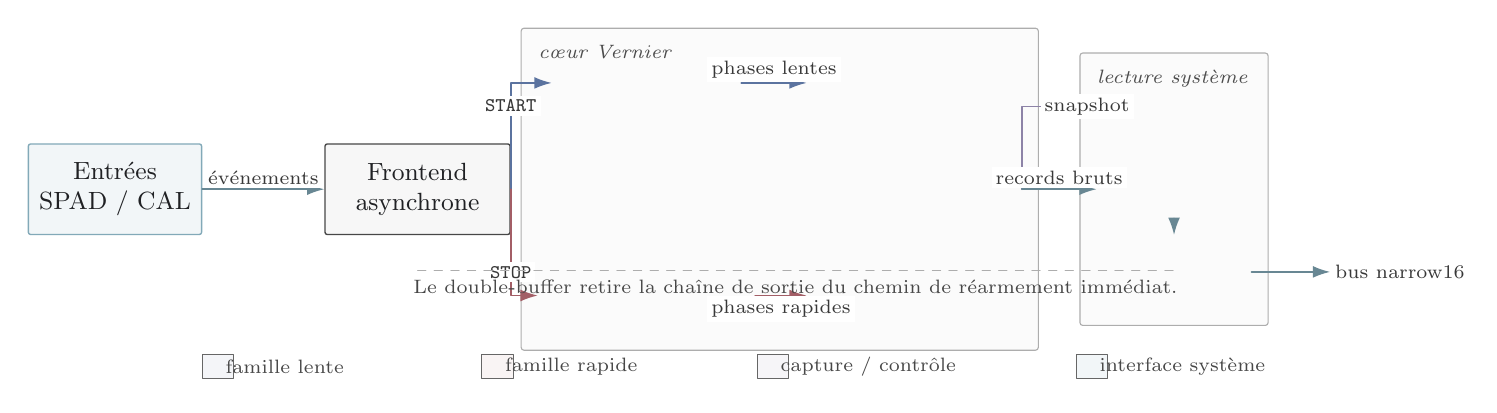
\begin{tikzpicture}[x=1cm,y=1cm]
  \node[module io, minimum width=2.20cm, minimum height=1.15cm] (inputs) at (0.0,0.0) {Entrées\\SPAD / CAL};
  \node[module gray, minimum width=2.35cm, minimum height=1.15cm, right=1.55cm of inputs] (frontend) {Frontend\\asynchrone};

  \node[module slow, minimum width=2.10cm, minimum height=0.95cm] (slowosc) at (6.75,1.35) {Oscillateur lent};
  \node[module fast, minimum width=2.10cm, minimum height=0.95cm] (fastosc) at (6.75,-1.35) {Oscillateur rapide};
  \node[module gray, minimum width=2.35cm, minimum height=1.35cm] (pd) at (10.15,0.0) {Matrice PD $9\times9$\\et capture fine};

  \node[module ctrl, minimum width=1.95cm, minimum height=0.92cm] (ctx) at (13.45,1.05) {Contextes\\$\times 2$};
  \node[module io, minimum width=1.95cm, minimum height=0.92cm] (drain) at (13.45,0.0) {Drain\\+ FIFO};
  \node[module io, minimum width=1.95cm, minimum height=0.92cm] (tx) at (13.45,-1.05) {TX\\\SI{16}{bit}};

  \node[domain box, fit=(slowosc)(fastosc)(pd), inner sep=6pt] (corefit) {};
  \node[domain box, fit=(ctx)(drain)(tx), inner sep=6pt] (iofit) {};
  \DomainLabel{corefit}{cœur Vernier}
  \DomainLabel{iofit}{lecture système}

  \draw[signal io] (inputs.east) -- node[note, above] {événements} (frontend.west);
  \draw[signal slow] (frontend.east) |- node[note, pos=0.34, above] {\texttt{START}} (slowosc.west);
  \draw[signal fast] (frontend.east) |- node[note, pos=0.34, below] {\texttt{STOP}} (fastosc.west);
  \draw[signal slow] (slowosc.east) -- node[note, above] {phases lentes} (pd.west|-slowosc.east);
  \draw[signal fast] (fastosc.east) -- node[note, below] {phases rapides} (pd.west|-fastosc.east);
  \draw[signal ctrl] (pd.east) |- node[note, pos=0.62, right] {snapshot} (ctx.west);
  \draw[signal io] (pd.east) -- node[note, above] {records bruts} (drain.west);
  \draw[signal io] (drain.south) -- (tx.north);
  \draw[signal io] (tx.east) -- ++(1.00,0) node[note, right] {bus narrow16};

  \draw[guide dashed] ($(frontend.south)+(0,-0.45)$) -- ($(frontend.south)+(9.6,-0.45)$);
  \node[axis label, anchor=north] at ($(frontend.south)+(4.80,-0.45)$)
    {Le double-buffer retire la chaîne de sortie du chemin de réarmement immédiat.};

  \LegendItem{(1.10,-2.25)}{TdcBlueFill}{TdcBlue}{famille lente}
  \LegendItem{(4.65,-2.25)}{TdcRedFill}{TdcRed}{famille rapide}
  \LegendItem{(8.15,-2.25)}{TdcLilacFill}{TdcLilac}{capture / contrôle}
  \LegendItem{(12.20,-2.25)}{TdcCyanFill}{TdcCyan}{interface système}
\end{tikzpicture}
\end{document}
